%==============================================================================
% locality-implementation.tex
%==============================================================================

\chapter{Implementation}
\label{chap:locality-implementation}

In this chapter we describe our new implementation of the intervals
scheduler. It is designed for locality-aware scheduling using locality
hints provided by the programmer.

INTRODUCTION


Instead of using work-stealing workers our design uses work-stealing
places. Section \ref{sec:locality-implementation-work-stealing-places}
presents the idea and implementation of work-stealing places. The
intervals scheduler implements each worker as a separate Java
thread. For the locality-aware scheduler we need to bind each worker
thread to a separate core. In Section
\ref{sec:locality-implementation-core-affinity} we show how we can set
the core affinity of Java threads. The API to use locality-awareness
in intervals is introduced in Section
\ref{sec:locality-implementation-intervals-api}.


\section{Work-Stealing Places}
\label{sec:locality-implementation-work-stealing-places}

A work-stealing scheduler employs a fixed number of threads called
workers. In traditional work-stealing scheduler designs, each worker
has a local double-ended queue, or deque, to maintain its own pool of
ready tasks from which it obtains work. We use so-called
\emph{Work-Stealing Places} instead. Each work-stealing place has a
local deque used to maintain ready tasks and a fixed number of
workers. The workers of a place share its local deque from which they
obtain work. When a worker finds that its place's pool is empty, it
becomes a thief and steals a task from the pool of a victim place
chosen at random.

Figure \ref{fig:locality-implementation-work-stealing-places} shows
the places used in our Intel Nehalem testing machine (Section
\ref{sec:experimental-setup-mafushi}).

\begin{figure}[!ht]
  \centering
  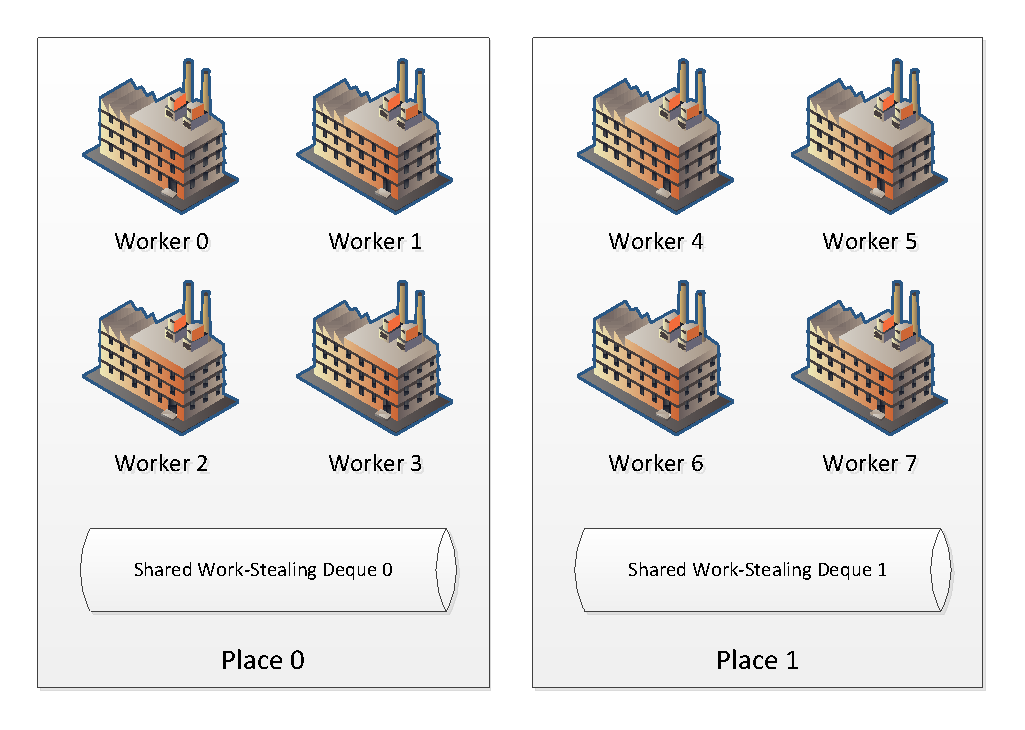
\includegraphics[width=\linewidth]{locality-implementation/places}
  \caption{Work-Stealing Places}
  \label{fig:locality-implementation-work-stealing-places}
\end{figure}

Our experiments with work-stealing queues showed that 

\todo{Finish section ``Work-Stealing Places''}


\section{Setting Core Affinity of Java Threads}
\label{sec:locality-implementation-core-affinity}

In recent Java Virtual Machines, threads are implemented with native
threads, so a Java program using threads is no different from a native
program using threads: A Java thread is just a thread belonging to a
JVM process. This means there is a 1-to-1 correspondence between Java
and native threads. When using the GNU C library on Linux, native
threads are implemented with the NPTL (Native POSIX Threads
Library). NPTL is also an 1-to-1 implementation, meaning that each
thread maps to a kernel scheduling entity (Figure
\ref{fig:locality-implementation-core-affinity-thread-mapping}).

\begin{figure}[htb]
  \centering
  \begin{tikzpicture}
    [node distance=0.8cm,
    start chain=going below,]
    \node[box, join] {Java Thread};
    \node[box, join] {Native POSIX Thread};
    \node[box, join] {Kernel Scheduling Entity};
  \end{tikzpicture}
  \caption{Linux 1-to-1 thread mapping}
  \label{fig:locality-implementation-core-affinity-thread-mapping}
\end{figure}

Unfortunately the Java Threads API does not expose the ability to set
the CPU or core affinity despite numerous use cases where setting the
affinity of threads would be beneficial -- such as improving cache and
network performance or real-time applications \cite{Love2003, Dow2005,
  Foong2008}. There exists a request for enhancement on this issue but
it got set to the state \emph{``Closed, Will Not Fix''}
\cite{Oracle1999}.

\subsection{JNI Library}
\label{sec:locality-implementation-core-affinity-jni-library}

To bind the workers to a specific core, we wrote a small JNI library
-- see Listing \ref{lst:locality-implementation-core-affinity} for the
API. The method \lstinline!set(int physicalUnit)!  (Line
\ref{lst:locality-implementation-core-affinity-set-unit}) is used to
bind the current thread to a physical unit. With
\lstinline!set(int[] physicalUnits)! the current thread can be bound
to several physical units, for example to a node in a NUMA system
(Line \ref{lst:locality-implementation-core-affinity-set-node}). For
debugging purposes we also implemented the method \lstinline!get()!
which returns a boolean array whose elements are true if the current
thread has an affinity set to the corresponding physical unit (Line
\ref{lst:locality-implementation-core-affinity-get}).

\lstinputlisting[style=FloatNumbers,
  caption={\lstinline{Affinity} class with interface for the native methods}, 
  label=lst:locality-implementation-core-affinity]{
    ../listings/locality-implementation/Affinity.java 
}

Listing \ref{lst:locality-implementation-core-affinity-jni-header}
contains the native method declarations which are implemented in
Listing \ref{lst:locality-implementation-core-affinity-jni-set} and
\ref{lst:locality-implementation-core-affinity-jni-get}. Line
\ref{lst:locality-implementation-core-affinity-jni-h-set-unit}
declares \lstinline!set(int physicalUnit)!. On Line
\ref{lst:locality-implementation-core-affinity-jni-h-set-node} we
declare the method \lstinline!set(int[] physicalUnits)! and
\lstinline!get()! is declared on Line
\ref{lst:locality-implementation-core-affinity-jni-h-get}.

\lstinputlisting[style=FloatNumbersC, 
  caption={\lstinline{Affinity} class: JNI C header}, 
  label=lst:locality-implementation-core-affinity-jni-header]{
    ../listings/locality-implementation/ch_ethz_hwloc_Affinity.h 
}

\lstinputlisting[style=FloatNumbersC, 
  caption={\lstinline{Affinity} class: JNI C implementation to set the affinity},
  label=lst:locality-implementation-core-affinity-jni-set]{
    ../listings/locality-implementation/ch_ethz_hwloc_Affinity_set.c 
}

The implementation for setting the affinity is shown in Listing
\ref{lst:locality-implementation-core-affinity-jni-set}. When setting
the affinity, we first initialize the CPU set structure (Lines
\ref{lst:locality-implementation-core-affinity-jni-set-unit-init-cpuset}
and
\ref{lst:locality-implementation-core-affinity-jni-set-node-init-cpuset})
and then we set it to the specified physical units (Lines
\ref{lst:locality-implementation-core-affinity-jni-set-unit-set-cpuset}
and
\ref{lst:locality-implementation-core-affinity-jni-set-node-set-cpuset}). The
actual setting of the affinity is done in function
\lstinline!set_affinity()! on Lines
\ref{lst:locality-implementation-core-affinity-jni-set-impl-start} --
\ref{lst:locality-implementation-core-affinity-jni-set-impl-end}.

To get the thread ID, we use the \lstinline!pthread_self()! function
(line
\ref{lst:locality-implementation-core-affinity-jni-set-impl-pthread-self}). The
function \lstinline!pthread_setaffinity_np()! (Line
\ref{lst:locality-implementation-core-affinity-jni-set-impl-set}) sets
the CPU affinity mask of the thread to the CPU set pointed to by
\lstinline!cpuset!.  If the call is successful, and the thread is not
currently running on one of the CPUs in \lstinline!cpuset!, then it is
migrated to one of those CPUs. If there is an error,
\lstinline!pthread_setaffinity_np()!  returs a nonzero error number
and we throw an exception (Line
\ref{lst:locality-implementation-core-affinity-jni-set-impl-set-error}).

Listing \ref{lst:locality-implementation-core-affinity-jni-get} shows
the implementation for getting the affinity of a thread. This method
is mainly used for debugging purposes. We use
\lstinline!pthread_self()! (Line
\ref{lst:locality-implementation-core-affinity-jni-get-impl-pthread-self})
to get the thread ID and then call function
\lstinline!pthread_getaffinity_np()!  (Line
\ref{lst:locality-implementation-core-affinity-jni-get-impl-get}). The
\lstinline!pthread_getaffinity_np()! function returns the CPU affinity
mask of the thread thread in the buffer pointed to by
\lstinline!cpuset!.

\lstinputlisting[style=FloatNumbersC, 
  caption={\lstinline{Affinity} class: JNI C implementation to get the affinity},
  label=lst:locality-implementation-core-affinity-jni-get]{
    ../listings/locality-implementation/ch_ethz_hwloc_Affinity_get.c 
}

\subsection{Restrictions}
\label{sec:locality-implementation-core-affinity-restrictions}

\subsubsection{Portability}

As we are directly using functions provided by POSIX threads, our
implementation is not portable across operating systems that do not
support the POSIX standard. To make our library portable, it could be
rewritten using \emph{Portable Linux Processor Affinity (PLPA)}
\cite{OpenMPI2010a} or \emph{Portable Hardware Locality (hwloc)}
\cite{OpenMPI2010}.

\subsubsection{Data Locality}

By setting the core affinity of threads, we only control the locality
of the work but we do not have control over data locality.

On a NUMA system every processor in the system has a local memory that
provides low access latency and high bandwidth, and a remote memory
that is considerably slower to access.

In the Java HotSpot VM, the NUMA-aware allocator has been implemented
to provide automatic memory placement optimisations for Java
applications \cite{Masamitsu2008, Oracle2010, Humble2010}: The
allocator controls the eden space of the young generation of the heap,
where most of the new objects are created. It divides the space into
regions each of which is placed in the memory of a specific node. The
allocator relies on a hypothesis that a thread that allocates the
object will be the most likely to use the object. To ensure the
fastest access to the new object, the allocator places it in the
region local to the allocating thread.

On Linux, the implementation is based on \cite{Kleen2004}. It can be
enabled by using the option \verb!-XX:+UseNUMA!.


\section{Intervals API}
\label{sec:locality-implementation-intervals-api}

\todo{Finish section ``Intervals API''}


\section{References}
\label{sec:locality-implementation-references}

The affinity of the workers is set such that they execute on different
cores. While this eliminates interference between the worker threads,
they will nevertheless share their assigned core with other processes
in the system, subject to standard Linux scheduling policy.

\subsection*{Intel threading building blocks: outfitting C++ for
  multi-core processor parallelism \cite{Reinders2007}}

\subsubsection{Caches}

The speed of processors has grown to be much faster than main
memory. Making all of memory nearly as fast as a processor would
simply prove too expensive for most computers. Instead, designers make
small amounts of memory, known as caches, operate nearly as fast as
the processor. The main memory can then be slower and more
affordable. The hardware knows how to move information in and out of
caches as needed, thereby adding to the number of places where data is
shuffled on its journey between memory and the processor cores. Caches
are critical in helping overcome the mismatch between memory speed and
processor speed.

Virtually all computers use caches only for a temporary copy of data
that should eventually reside in memory. Therefore, the function of a
memory subsystem is to move data needed as input by each processing
core to caches near that processor core, and to move data produced by
the processing cores out to main memory. As data is read from memory
into the caches, some data needs to be evicted from the cache. Cache
designers work to make the data evicted be approximately the data
least likely to be used again.

Once a processor accesses data, it is best to exhaust the program’s
use of it while it is still in the cache. Continued usage will hold it
in the cache, whereas prolonged inactivity will likely lead to its
eviction and future usage will need to do a more expensive (slow)
access to get the data. Furthermore, every time an additional thread
runs on a processor core, data is likely to be discarded from the
cache.

Threading Building Blocks is designed with caches in mind and works to
limit the unnecessary movement of tasks and data. When a task has to
be passed to a different processor core for execution, Threading
Building Blocks moves the task with the least likelihood of having
data in the cache for the processor core from which the task is
stolen.

It is interesting to note that parallel Quicksort (Chapter 11) is an
example in which caches beat maximum parallelism. Parallel Mergesort
has more parallelism than parallel Quicksort. But parallel Mergesort
is not an in-place sort, and thus has twice the cache footprint that
parallel Quicksort does. Hence, Quicksort usually runs faster in
practice.

Keep data locality in mind when considering how to structure your
program. Avoid using data regions sporadically when you can design the
application to use a single set of data in focused chunks of
time. This happens most naturally if you use data decomposition,
especially at the higher levels in a program.

\subsubsection{Costs of Time Slicing}

Time slicing enables there to be more logical threads than physical
threads. Each logical thread is serviced for a time slice—a short
period of time defined by the operating system during which a thread
can run before being preempted—by a physical thread. If a thread runs
longer than a time slice, as most do, it relinquishes the physical
thread until it gets another turn. This chapter details the costs
incurred by time slicing.

The most obvious cost is the time for context switching between
logical threads. Each context switch requires that the processor save
all its registers for the previous logical thread that it was
executing, and load its registers with information for the next
logical thread it runs.

A subtler cost is cache cooling. Processors keep recently accessed
data in cache memory, which is very fast, but also relatively small
compared to main memory. When the processor runs out of cache memory,
it has to evict items from cache and put them back into main
memory. Typically, it chooses the least recently-used items in the
cache. (The reality of set-associative caches is a bit more
complicated, but this is not a cache primer.)

When a logical thread gets its time slice, as it references a piece of
data for the first time, this data is pulled into cache, taking
hundreds of cycles. If it is referenced frequently enough not to be
evicted, each subsequent reference will find it in cache, and take
only a few cycles. Such data is called hot in cache.

Time slicing undoes this because if Thread A finishes its time slice,
and subsequently Thread B runs on the same physical thread, B will
tend to evict data that was hot in cache for A, unless both threads
need the data. When Thread A gets its next time slice, it will need to
reload evicted data, at the cost of hundreds of cycles for each cache
miss. Or worse yet, the next time slice for Thread A may be on a
different physical thread that has a different cache altogether.

Another cost is lock preemption. This happens if a thread acquires a
lock on a resource and its time slice runs out before it releases the
lock. No matter how short a time the thread intended to hold the lock,
it is now going to hold it for at least as long as it takes for its
next turn at a time slice to come up. Any other threads waiting on the
lock either busy-wait pointlessly or lose the rest of their time
slice. The effect is called convoying because the threads end up
``bumper to bumper'' waiting for the preempted thread in front to resume
driving.

\todo{Finish chapter ``Implementation''}


%%% Local Variables: 
%%% mode: latex
%%% TeX-master: "thesis"
%%% End: 
